\section{Explainable AI}
\subsection{Interpretability}
L'obiettivo è sempre quello di capire il perchè una macchina riesce ad imparare dai dati. Vogliamo quindi motivare perchè un algoritmo sceglie in un certo modo. 
\\
\textbf{Ma perchè non lasciare decidere al modello e fregarsene?} Uno dei principali motivi è la fairness. Un modello che decide uomo e donna, bianco o nero\dots il modello deve generalizzare ma soprattutto deve evitare razzismo, omofobia, misoginia. Se capiamo il motivo dietro alle sue scelte, possiamo influenzarle. Si distinguono:
\begin{itemize}
    \item modelli intrinsic: modelli ultra interpretabili, come gli alberi
    \item modelli post hoc., modelli aggiuntivi, cioè io ho dei modelli non interpretabili che mi danno l'accuracy e dei modelli semplici che spiegano quelli non interpretabili 
\end{itemize}
Come risultati dell'interpretazione otteniamo:
\begin{itemize}
    \item feature summary statistic: una statistica per ogni feature
    \item model internals: per esempio dei weights
    \item data points: categoria che identifica tutte le tecniche che danno come risultato dei data points per l'interpretabilità
    \item intrinsecally interpretable model: approssimare un modello black box con uno white box
\end{itemize}
E si possono distinguere anche tra spiegazione globale e locale, dove una ovviamente spiega a livello generale un modello mentre l'altra è sulla singola predizione. Poi ci sono diverse metriche per la valutazione della spiegazione, come l'accuracy e la fedeltà. La fedeltà è molto importante perchè rappresenta quanto la spiegazione è corretta. Ovvero quanto il modello utilizzato riesce a rappresentare il modello più complicato.
\\
Algoritmi diversi, danno pesi diversi. Quindi un altro problema da porci è la consistency insieme alla stability. Ovviamente la spiegazione dev'essere ben diversificata sulla base dell'istanza, altrimenti non è comprensibile; e deve avere un certo grado di importanza per far capire l'importanza delle feature spiegate. 

\subsubsection{Interpretable Models}
\begin{itemize}
    \item \textbf{Linear regression:} molto semplice da capire perchè è un modello lineare la cui rappresentazione è una semplice retta. Tanto più il coefficiente è elevato, tanto più quel valore avrà importanza. La valutazione dell'importanza può essere fatta attraverso l'utilizzo delle Effect Plot, che si calcolano semplicemente come il peso per l'attributo. 
    \item \textbf{Logistic regression:} L'interpretazione non è semplice come nella linear regression, soprattutto parlando dei pesi. Il cambiamento di una feature di una unità, cambia il valore esponenzialmente (exp). 
    \item \textbf{Decision tree:} probabilmente il modello white box per eccellenza, una decisione binaria multipla, per capirlo basta "seguire il percorso che fa l'albero". Come faccio a dare più o meno importanza nella decisione di un nodo dell'albero? Guardiamo il calo di entropia (guardiamo l'info gain). 
\end{itemize}
Andiamo a vedere come funzionano i modelli agnostici globali. 

\newpage

\subsubsection{Partial Dependence Plot}
Mostra l'effetto marginale che hanno una o due features sulla prediction del modello ML. Sono dei diagrammi, che mostrano l'impatto sul risultato finale. 
\\
Si calcola con la feature di interesse e dei valori significativi per tale feature; fisso un valore significativo e cambio le altre feature: ad esempio, feature \texttt{Temperatura} valore significativo 10, fisso questo e cambio tutte le altre, poi faccio la prediction. Faccio la media dei risultati e costruisco i diagrammi. 
\begin{center}
    \begin{math}
        f_{S}(x_S) = \frac{1}{n} \sum_{i=1}^{n} f(x_S, x_C^{(i)})
    \end{math}
\end{center}
Ed è una spiegazione globale.

\subsubsection{Permutation Feature Importance}
Valutiamo se una feature è importante semplicemente guardando quanto cambia il risultato se modifico i valori che aveva in precedenza tale feature. 
\\
Torniamo sull'esempio precedente, \texttt{Temperatura}, e prendiamo tutti i suoi valori. Facciamo uno shuffle e li scambiamo. Come varia l'accuracy del modello? Se varia molto, allora la feature è molto importante altrimenti non lo è. 
\\
\begin{figure}[th]
    \centering
    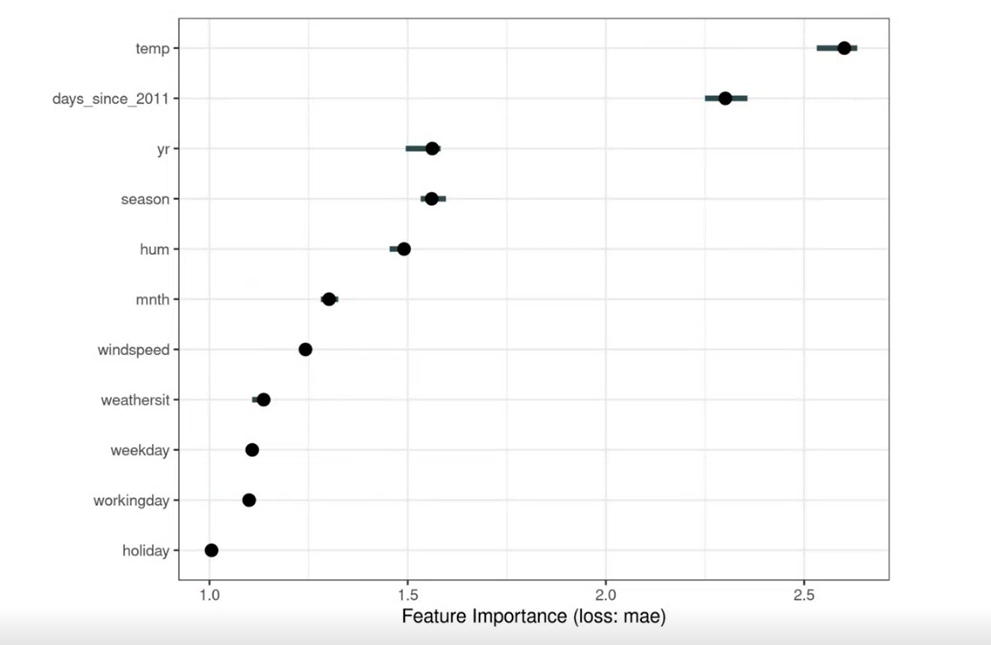
\includegraphics[scale=0.4]{ExplainableAI/img/pfi.png}
\end{figure}
\\
Questo è un possibile diagramma delle pfi di un dataset. Ed è sempre un discorso globale, perchè lo dico in funzione delle altre features. 
\\
\textbf{Attenzione!} Calcolare la pfi è un'operazione da fare nel test e non nel training, per evitare overfitting (che è molto presente durante il training). 

\subsubsection{Leave-One-Covariate-Out}
Alleno senza una feature e guardo come varia il risultato. Introduco una nuova grandezza: LOCO Feature Importance, come il rapporto tra l'errore sul dataset iniziale e quello senza la feature. Non otteniamo un diagramma, potremmo fare come per il permutation feature importance. 

\newpage 

\subsubsection{Local Surrogate (LIME)}
Modello agnostico locale. Si usa un po' ovunque. Costruisce un modello lineare che rappresenta un modello complesso, sulle singole prediction. Il modello surrogato non è uguale al modello complesso, ma nell'intorno considerato le prediction sono simili! 
\\
Costruiamo un nuovo dataset, creando una perturbazione del dataset originale. Individuiamo un valore di una feature, e lo sostiuiamo con valori in un suo intorno. Ottengo una label diversa! 
\\
Un altro modo potrebbe anche essere quello di eliminare delle features (ad esempio, per le feature categoriche). Più la perturbazione mi porta vicino, più è importante quindi sarà una perturbazione pesata. Uso un dataset perturbato con una funzione lineare e ottenere un risultato simile. 
\begin{center}
    \begin{math}
        explanation(x) = arg min L(f,g, \pi_x)+ \Omega(g)
    \end{math}
\end{center}
Questo è l'explanation model per x. Il valore in pi greco è la grandezza dell'intorno di x. 

\subsubsection{Counterfactual Explanation}
Altre spiegazioni a livello locale. Si può spiegare banalmente in questo modo: se mia nonna avesse avuto le ruote sarebbe stata una carriola. 
\\
Il ragionamento dietro alle counterfactual è di facile interpretazione per l'utente, perchè ipotizzo che se una delle feature fosse diversa, probabilmente sarebbe diverso anche il risultato della prediction. 
\\
Uno dei principali contro sarebbe il 'Rashomon effect': ci sono più motivi solitamente per cui una prediction cambia, quindi lo stesso caso potrebbe avere tante spiegazioni diverse. Inoltre potrei cambiare feature ipotizzando cose impossibili.
\\
Quindi riassumendo: modifico delle feature fino ad ottenere il risultato di prediction opposto. 

\subsubsection{Shapley Values}
Immaginiamo che ogni valore di feature sia semplicemente un 'giocatore' e la prediction il risultato del gioco. 
\\
\textit{Esempio.} Hai allenato un modello per predire il prezzo di un appartamento. Uno di essi, ha come prezzo previsto 300k. Questo appartamento ha certe features: area 50, secondo piano, parcheggio e gatti proibiti. In generale, il valore previsto per questi appartamenti sta sui 310k, quindi sei in perdita di 10k. Potremmo vedere le singole feature quanto tolgono dal prezzo, e questo spiegherebbe il prezzo finale. Ad esempio, il problema potrebbe essere la questione gatto, che potrebbe abbassare il prezzo dell'appartamento. 
\\
Devo quindi confrontarmi con le altre 'coalizioni' ovvero uso delle feature diverse e vedo la prediction come cambia. 
\\
I 4 \textbf{assiomi} del valore di Shapley:
\begin{itemize}
    \item \textbf{Efficienza:} tutti i ricavi della grande coalizione N sono da spartire tra tutte le features
    \item \textbf{Simmetria:} giocatore i e j che hanno lo stesso contributo, ottengono lo stesso ricavo 
    \item \textbf{Linearità:} i valori di due 'giochi' distinti si possono sommare linearmente
    \item \textbf{Dummy player:} Quelli che non contribuiscono non ottengono nulla 
\end{itemize}

\newpage

La \textbf{Shapley value equation:}
\begin{center}
    \begin{math}
        \phi_i(N,v) = \frac{1}{N!} \sum |S|!(|N|-|S|-1)! [v(S \cup \{ i\}) -v(S)]
    \end{math}
\end{center}
Dove la sommatoria su tutte le possibili coalizioni senza l'elemento che sto considerando. E l'ultimo termine sottraggo la coalizione con e senza l'elemento considerato. 
\\
\begin{figure}[th]
    \centering
    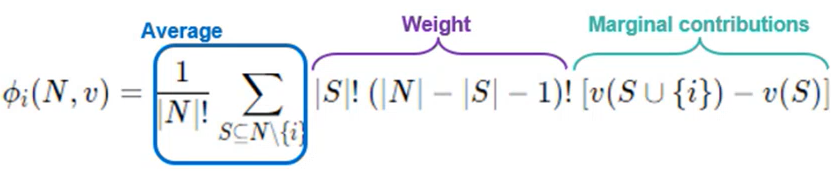
\includegraphics[scale=0.5]{ExplainableAI/img/shapley function.png}
\end{figure}
\\
Esistono un paio di modi per approssimare la Shapley, dato che è molto complessa da calcolare, come la SHAP che approssima il calcolo. 

\subsubsection{KernelSHAP}
Il valore nella SHAP fa una maschera (kernel) per quello prende il nome di kernelshap. Vediamo la formula nel dettaglio:
\begin{center}
    \begin{math}
        g(z') = \phi_0 + \sum_{j=1}^{M} \phi_j z_j'
    \end{math}
\end{center}
Dove z è il coalition vector, il vettore delle coalizioni, che è 0 o 1 e fa quindi una maschera. Facendo una maschera di fatto sto anche creando un nuovo dataset!
\\
Dopo aver applicato la maschera, peso ogni punto secondo questa formula: 
\\
\begin{figure}[th]
    \centering
    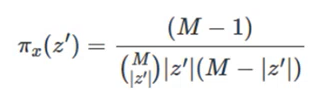
\includegraphics[scale=0.6]{ExplainableAI/img/weights.png}
\end{figure}
\\
Che vuol dire che se ho solo valori mascherati quella riga vale molto, se ne ho un po' non mascherati vale meno. Ora fitta il modello con i pesi di Shapley. 


